\section{Resultados}

\subsection{Estatísticas Descritivas}

A Tabela~\ref{tab:descritivas} apresenta as estatísticas descritivas do tempo
de resposta (ms) por tratamento.

\begin{table}[H]
\centering
\caption{Estatísticas descritivas do tempo de resposta (ms)}
\label{tab:descritivas}
\begin{tabular}{lrrrrrrr}
\toprule
Tratamento & Média & DP & Mín. & Q1 & Mediana & Q3 & Máx. \\
\midrule
REST & 189,60 & 41,09 & 69,12 & 164,78 & 190,69 & 216,22 & 263,96 \\
GraphQL & 246,25 & 48,84 & 154,52 & 208,47 & 240,23 & 273,56 & 362,70 \\
\bottomrule
\end{tabular}
\end{table}

\subsection{Testes de Hipóteses}

O teste de Shapiro-Wilk indicou normalidade nos dados ($p > 0,05$), portanto
foi utilizado o teste t de Student para RQ1. Para RQ2, foi utilizado o teste
de Wilcoxon-Mann-Whitney.

\begin{table}[H]
\centering
\caption{Resultados dos testes estatísticos}
\label{tab:testes}
\begin{tabular}{llll}
\toprule
RQ & Teste & Estatística & p-valor \\
\midrule
RQ1 (tempo) & t de Student & 4,86 & $> 0,999$ \\
RQ2 (bytes) & Wilcoxon-Mann-Whitney & 0,0 & $< 0,001$ \\
\bottomrule
\end{tabular}
\end{table}

\subsection{Visualizações}

\begin{figure}[H]
\centering
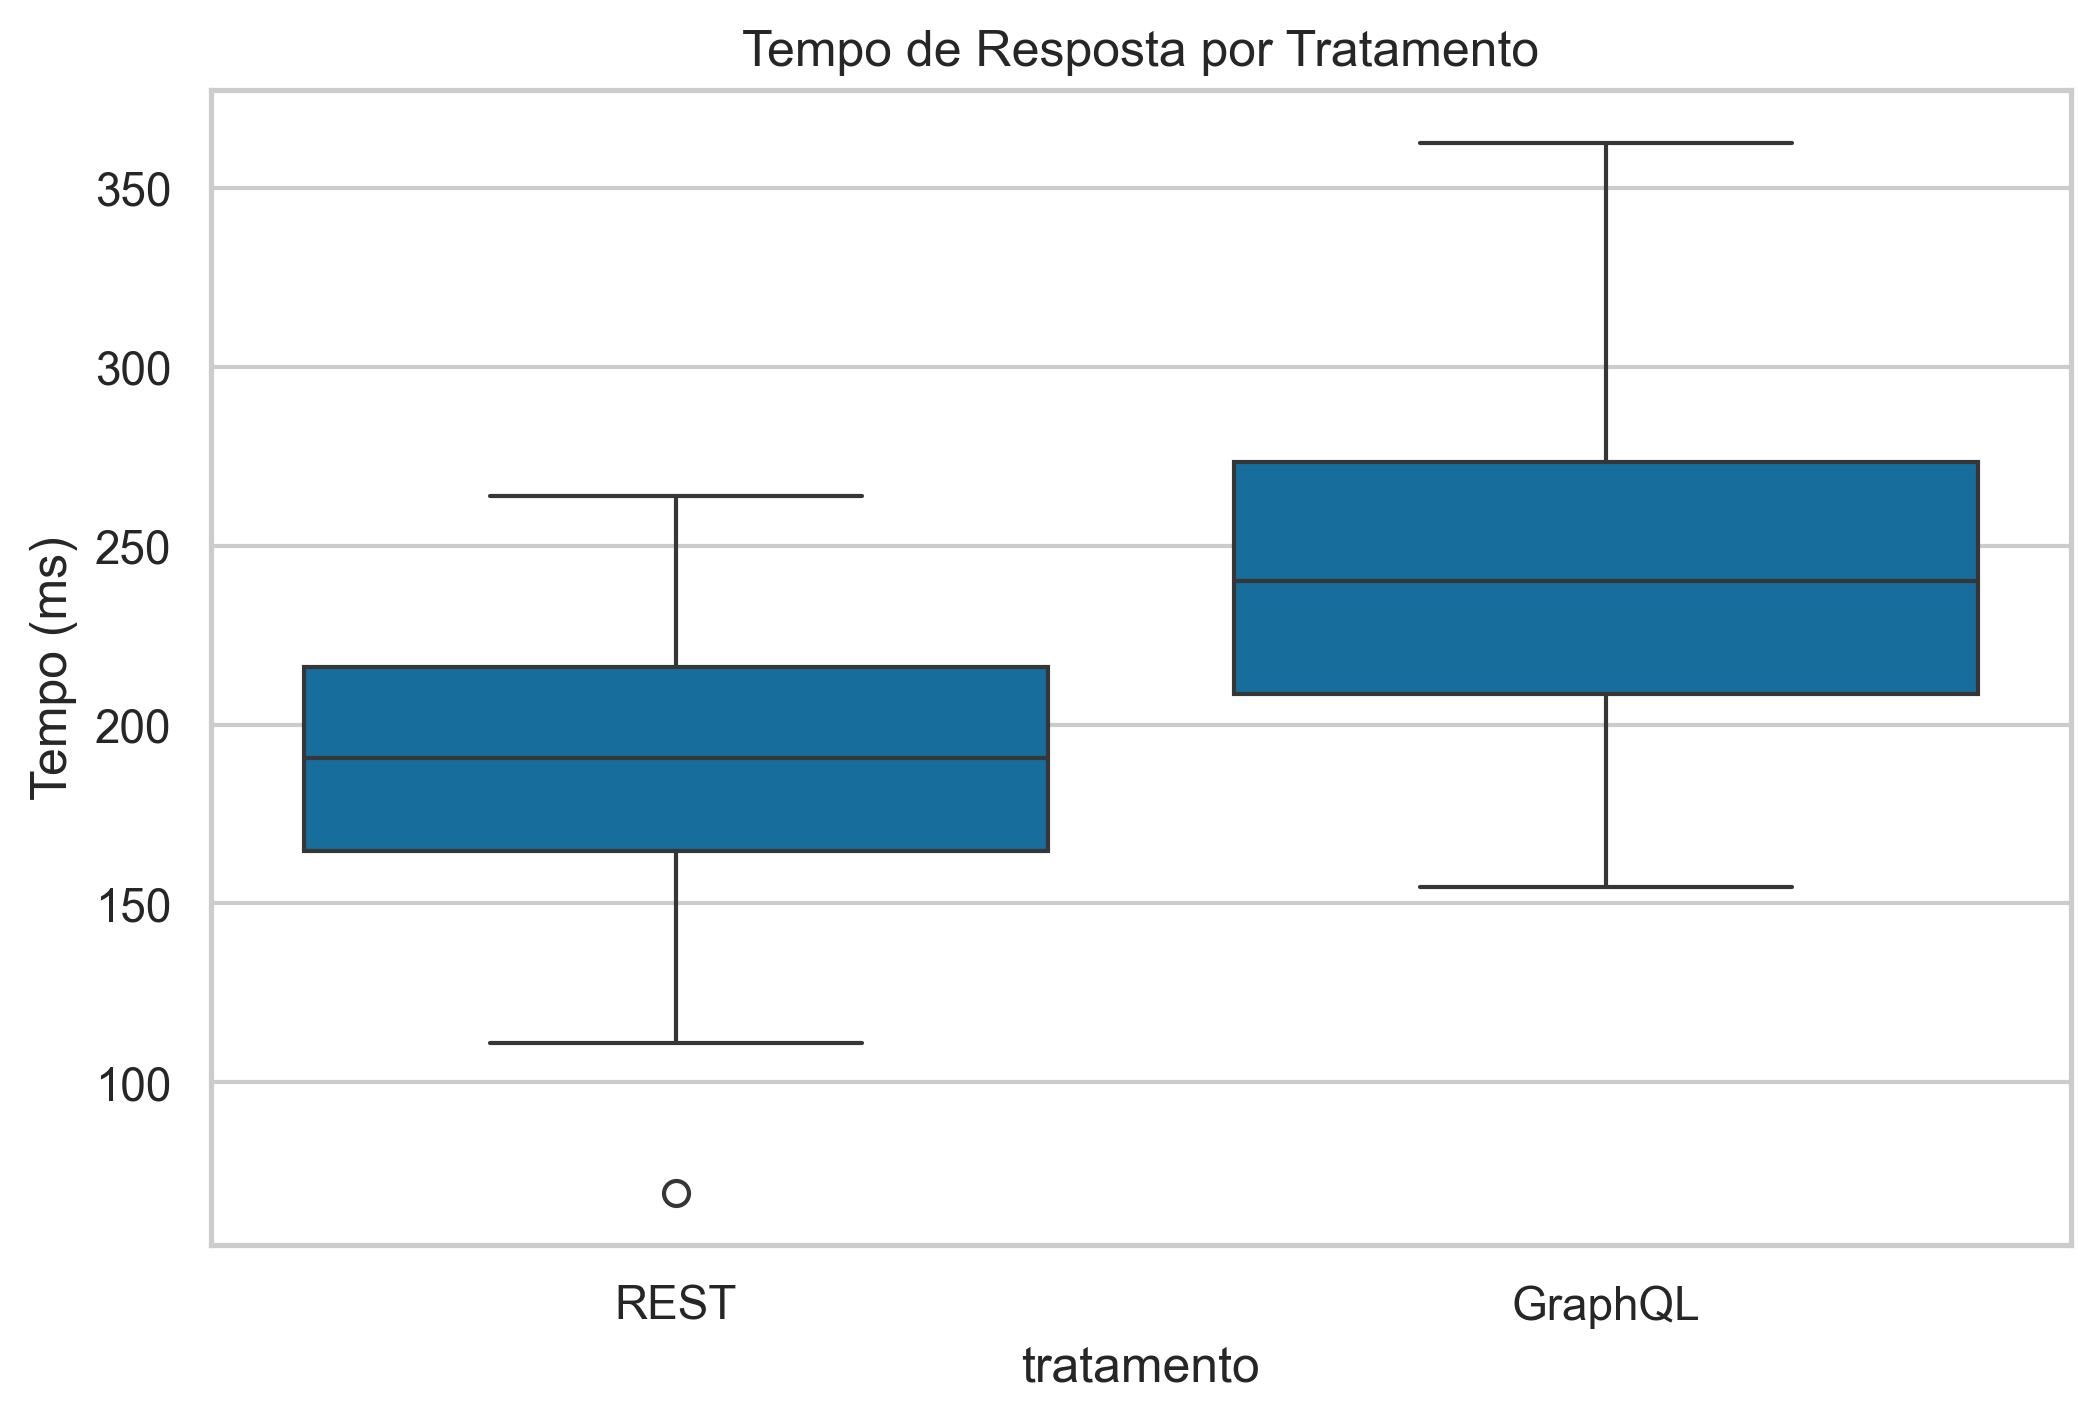
\includegraphics[width=0.8\textwidth]{figures/boxplot_tempo.png}
\caption{Tempo de resposta por tratamento}
\label{fig:boxplot_tempo}
\end{figure}

\begin{figure}[H]
\centering
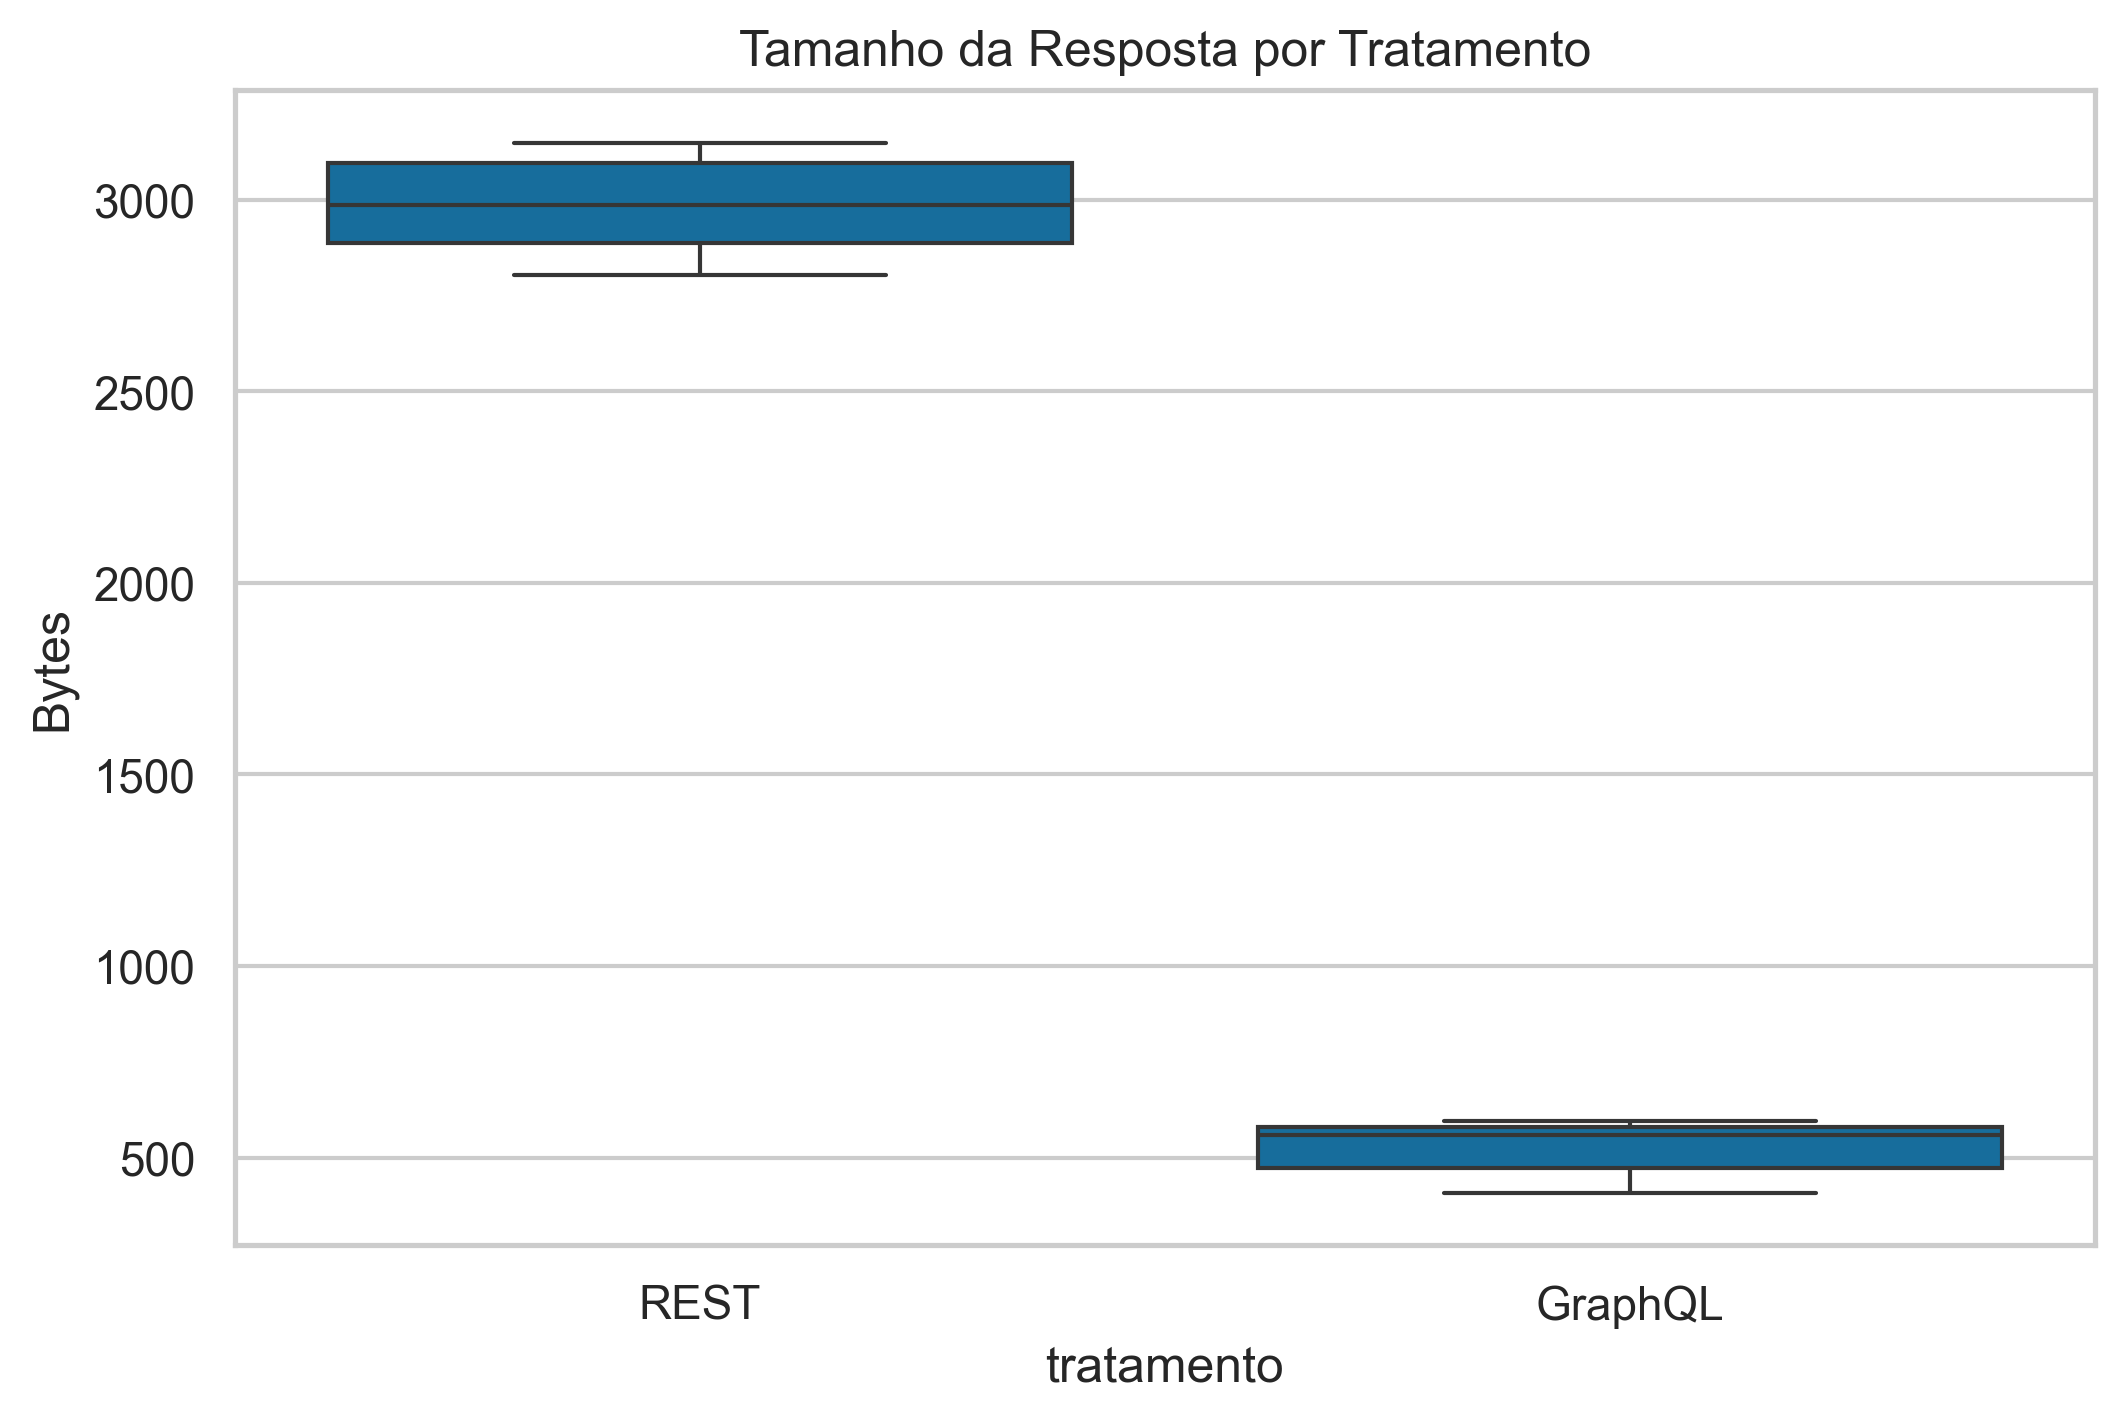
\includegraphics[width=0.8\textwidth]{figures/boxplot_bytes.png}
\caption{Tamanho da resposta por tratamento}
\label{fig:boxplot_bytes}
\end{figure}

\begin{figure}[H]
\centering
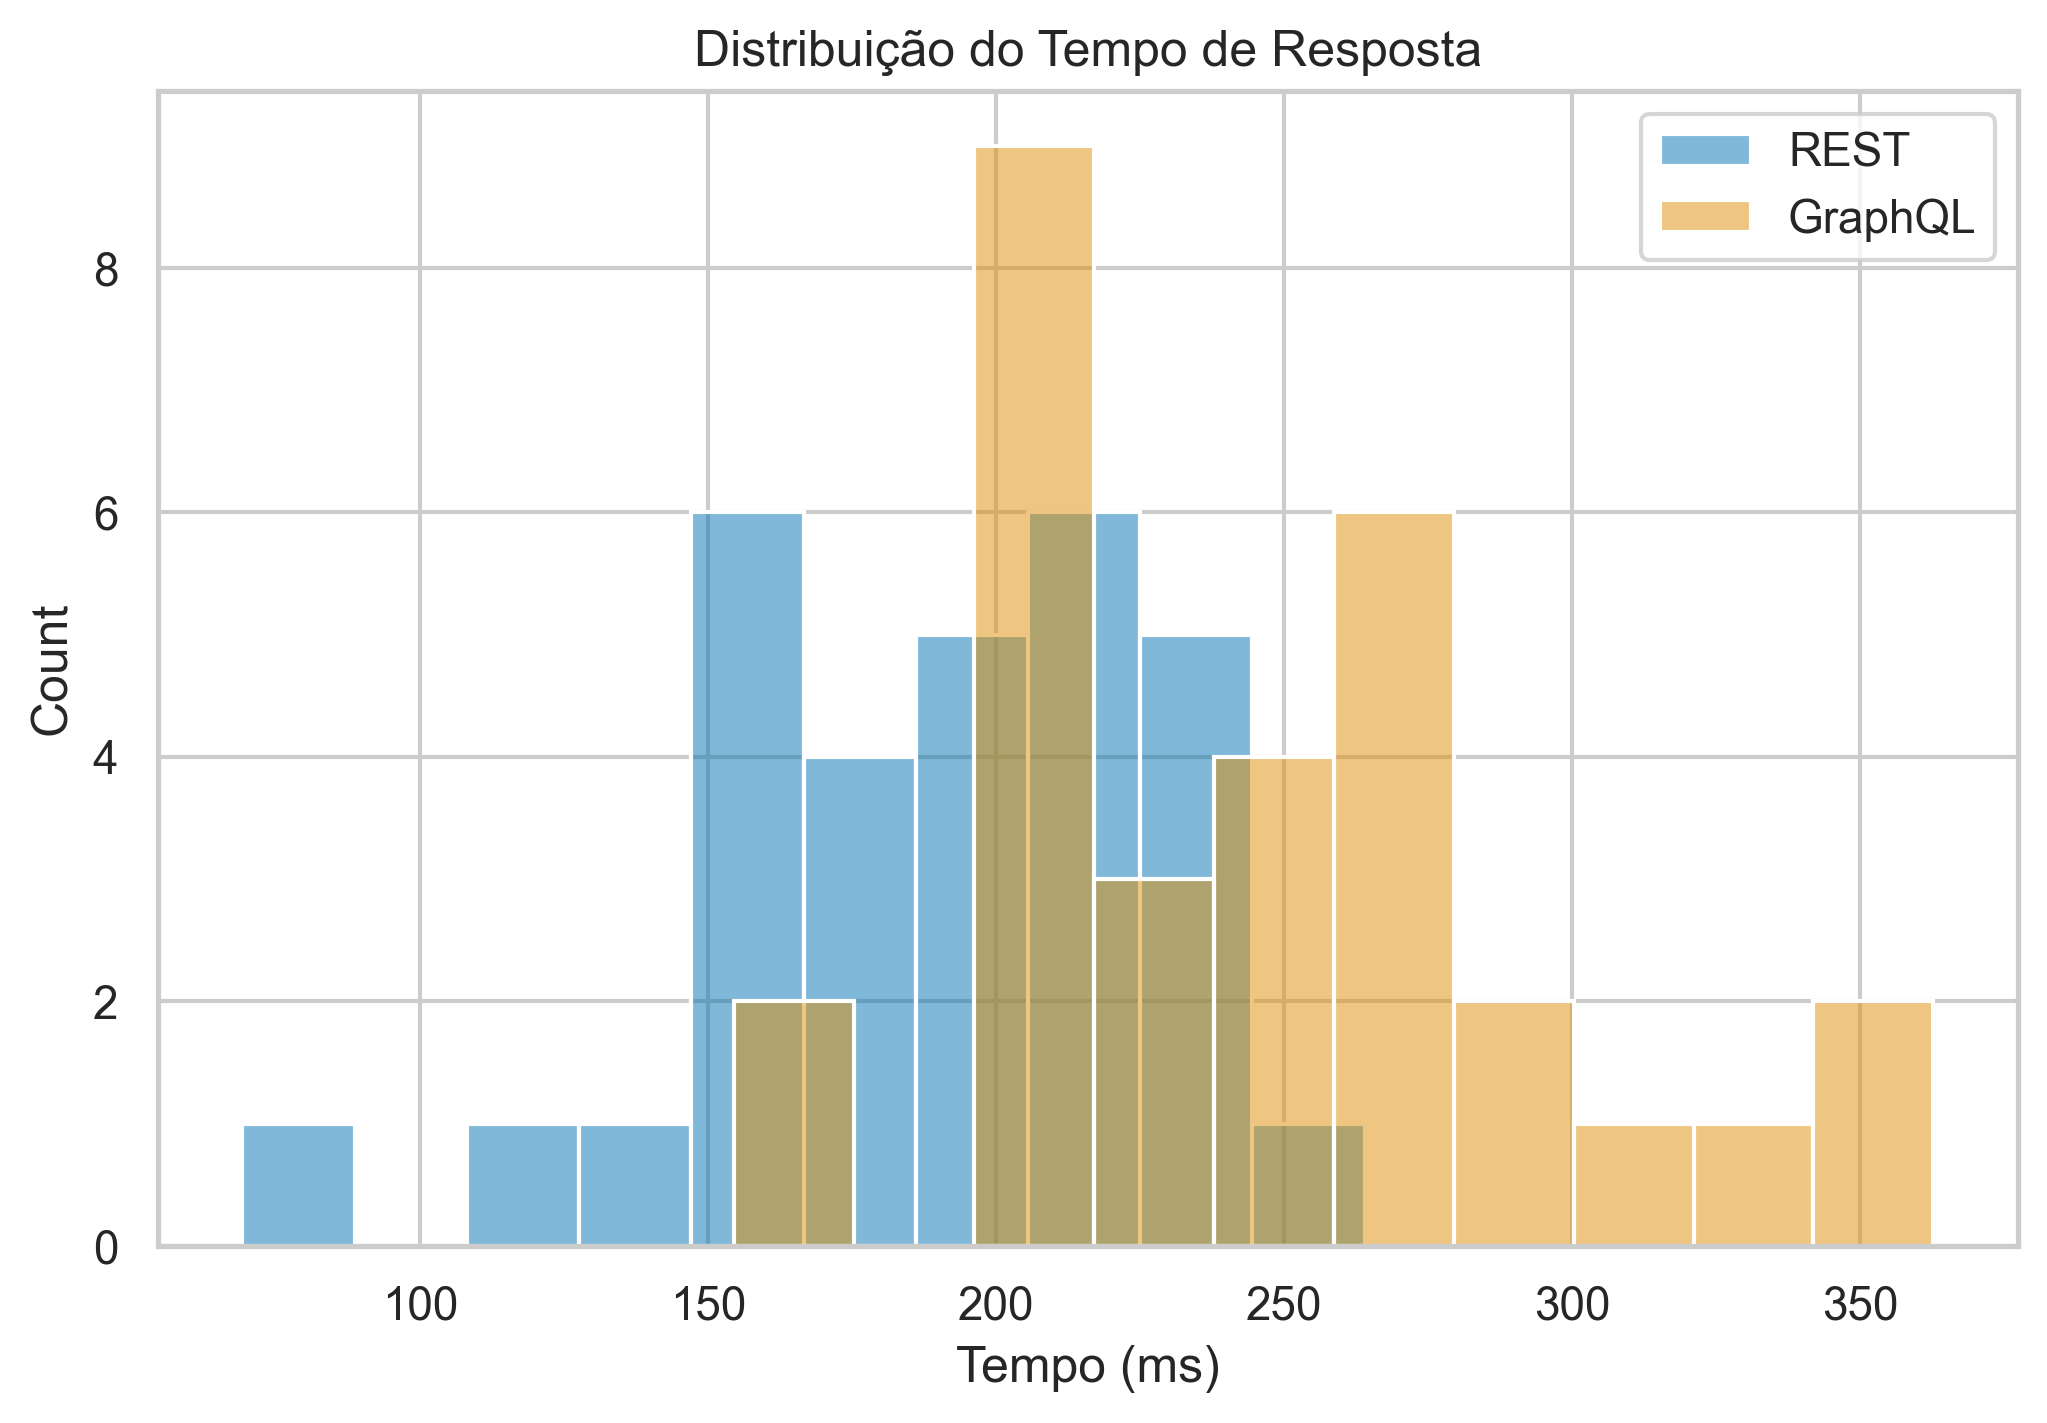
\includegraphics[width=0.8\textwidth]{figures/histograma_tempo.png}
\caption{Distribuição do tempo de resposta}
\label{fig:hist_tempo}
\end{figure}

\begin{figure}[H]
\centering
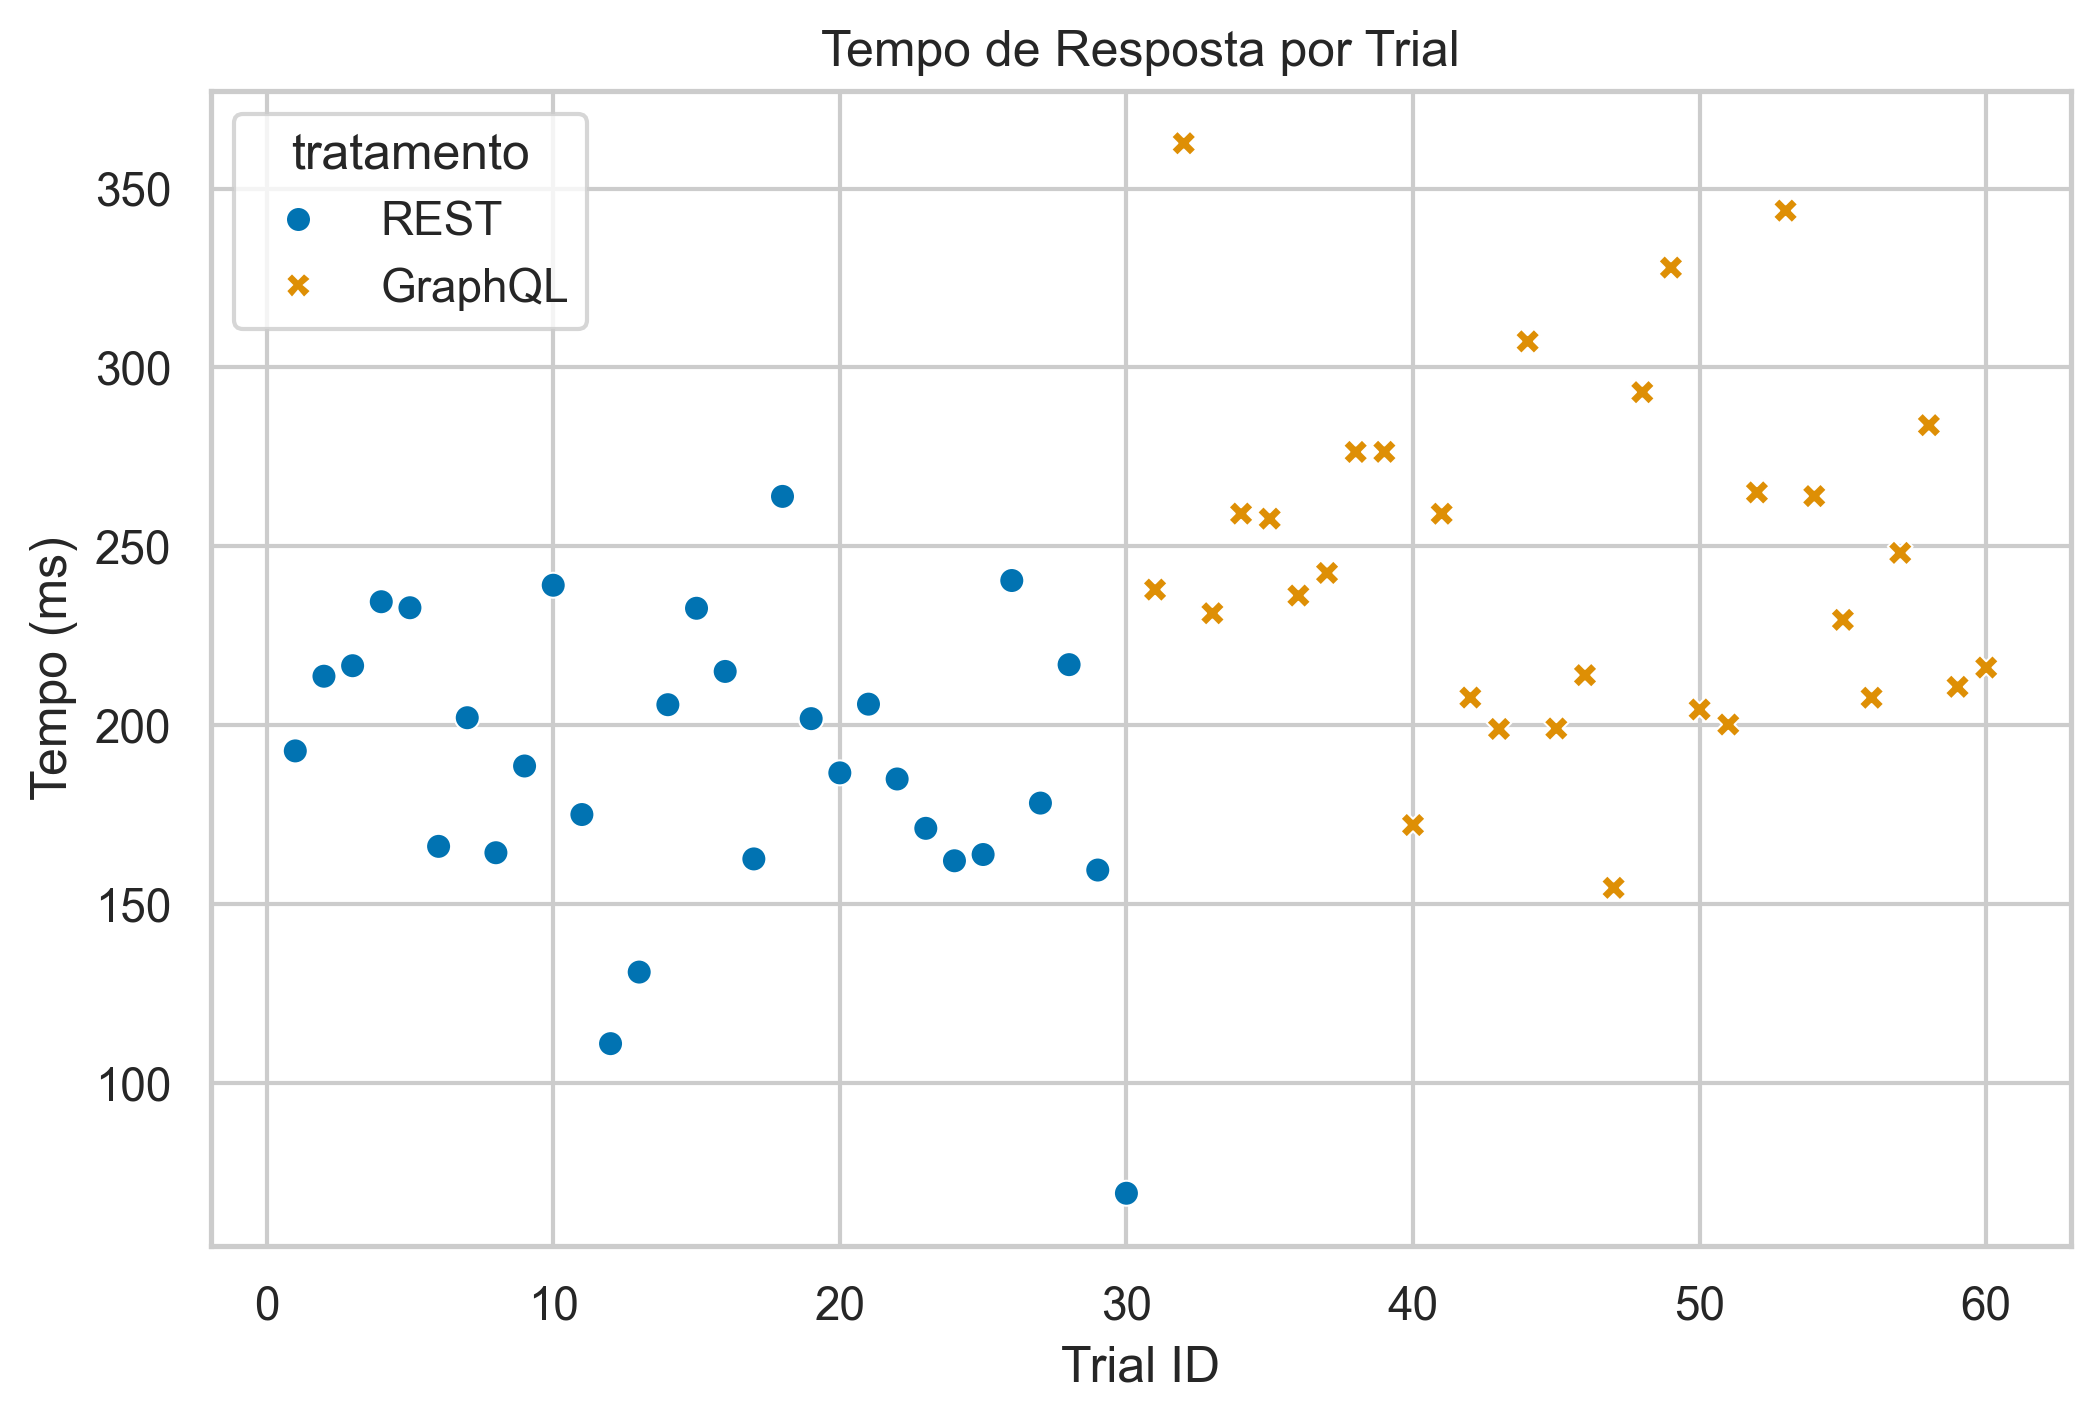
\includegraphics[width=0.8\textwidth]{figures/scatter_tempo.png}
\caption{Tempo de resposta por trial}
\label{fig:scatter_tempo}
\end{figure}
